\begin{figure}[t]
\centering
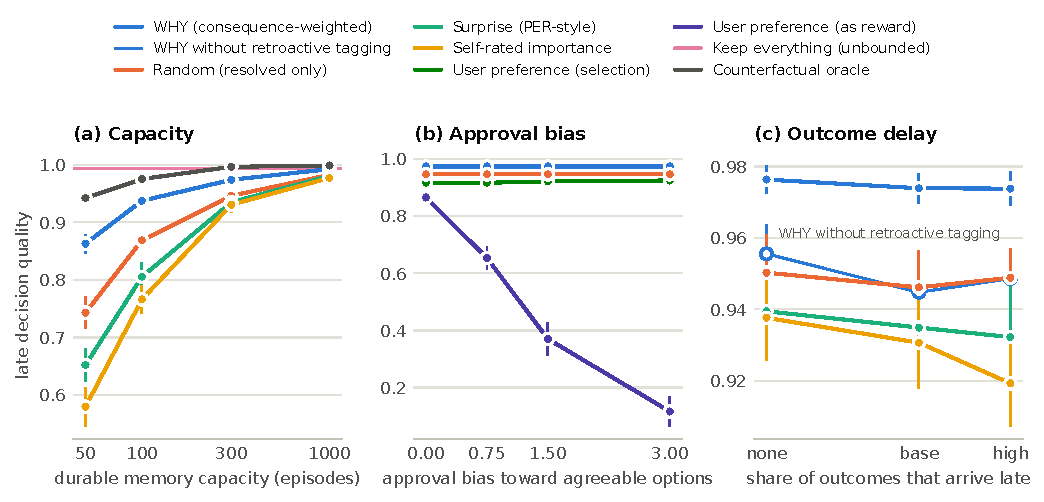
\includegraphics[width=\linewidth]{../figs/fig_sweeps.pdf}
\caption{Sweeps in the Realistic scenario (20 seeds, 95\% CIs). (a) Durable memory capacity; the horizontal line is unbounded memory. (b) Strength of the approval bias toward agreeable options. (c) Share of outcomes that resolve late (none, base rate, high). WHY and resolved-only random retention never read approval, so their lines in (b) are flat by construction.}
\label{fig:sweeps}
\end{figure}

\subsection{Capacity, approval, and delay}
\label{sec:sweeps}
\paragraph{Capacity.} The advantage of consequence-weighting grows as memory shrinks (Figure~\ref{fig:sweeps}a). At 50 engrams WHY reached \val{capsw-why-50}, against \val{capsw-random_resolved-50} for resolved-only random retention, \val{capsw-surprise-50} for PER-style surprise, and \val{capsw-importance-50} for self-rated importance. At 1{,}000 engrams, a sixth of all episodes, it reached \val{capsw-why-1000}, statistically indistinguishable from unbounded memory (\val{capsw-keep_all}; paired difference \val{pair-cap1000-keep_all}\,$\pm$\,\val{pair-cap1000-keep_all-ci}), while resolved-only random retention reached \val{capsw-random_resolved-1000}. The oracle's \val{capsw-oracle-50} at 50 engrams shows how much more a better selection rule could still recover when memory is scarce.

\paragraph{Approval bias.} Selecting episodes by approval cost roughly the same at every level of bias (\val{appr-user_pref-0.0} with no bias, \val{appr-user_pref-3.0} with strong bias), because that policy still trained on outcomes (Figure~\ref{fig:sweeps}b). Using approval as the reward collapsed as the bias grew, from \val{appr-user_pref_reward-0.0} to \val{appr-user_pref_reward-0.75}, \val{appr-user_pref_reward-1.5}, and \val{appr-user_pref_reward-3.0}. The damage comes from what a memory is trained on, more than from which memories are selected.

\paragraph{Delay.} WHY's decision quality barely moved as the share of late outcomes changed (\val{delay-why-0.0}, \val{delay-why-1.0}, \val{delay-why-1.6}; Figure~\ref{fig:sweeps}c), and neither did the value of retroactive tagging (\val{delay-retro_gap-0.0}, \val{delay-retro_gap-1.0}, \val{delay-retro_gap-1.6}). In this environment its value comes less from late outcomes specifically than from refusing to commit before any outcome exists, including the fifth of outcomes that never arrive, and from rescoring as the model changes. Self-rated importance, which commits at write time, declined as delays grew (\val{delay-importance-0.0} to \val{delay-importance-1.6}).
